\subsection{Thiết kế Giao diện (User Interface Design)}

\textbf{Sơ đồ điều hướng màn hình (Windows Navigation Diagram)}
Sơ đồ điều hướng màn hình (WND) dưới đây mô tả luồng di chuyển và các sự kiện chuyển trang của hệ thống HomeStay Dorm. Sơ đồ phân tách rõ các phân hệ dành cho Khách truy cập (Public), Khách hàng (Customer) và Nhân sự vận hành (Admin), tuân thủ thiết kế Single Page Application (SPA) trên nền tảng Angular. Các thành phần được phân loại rõ ràng bao gồm: Cửa sổ (\texttt{<<Window>>}), Biểu mẫu (\texttt{<<Form>>}), Báo cáo (\texttt{<<Report>>}) và Hộp thoại (\texttt{<<Modal>>}).

\begin{figure}[H]
    \centering
    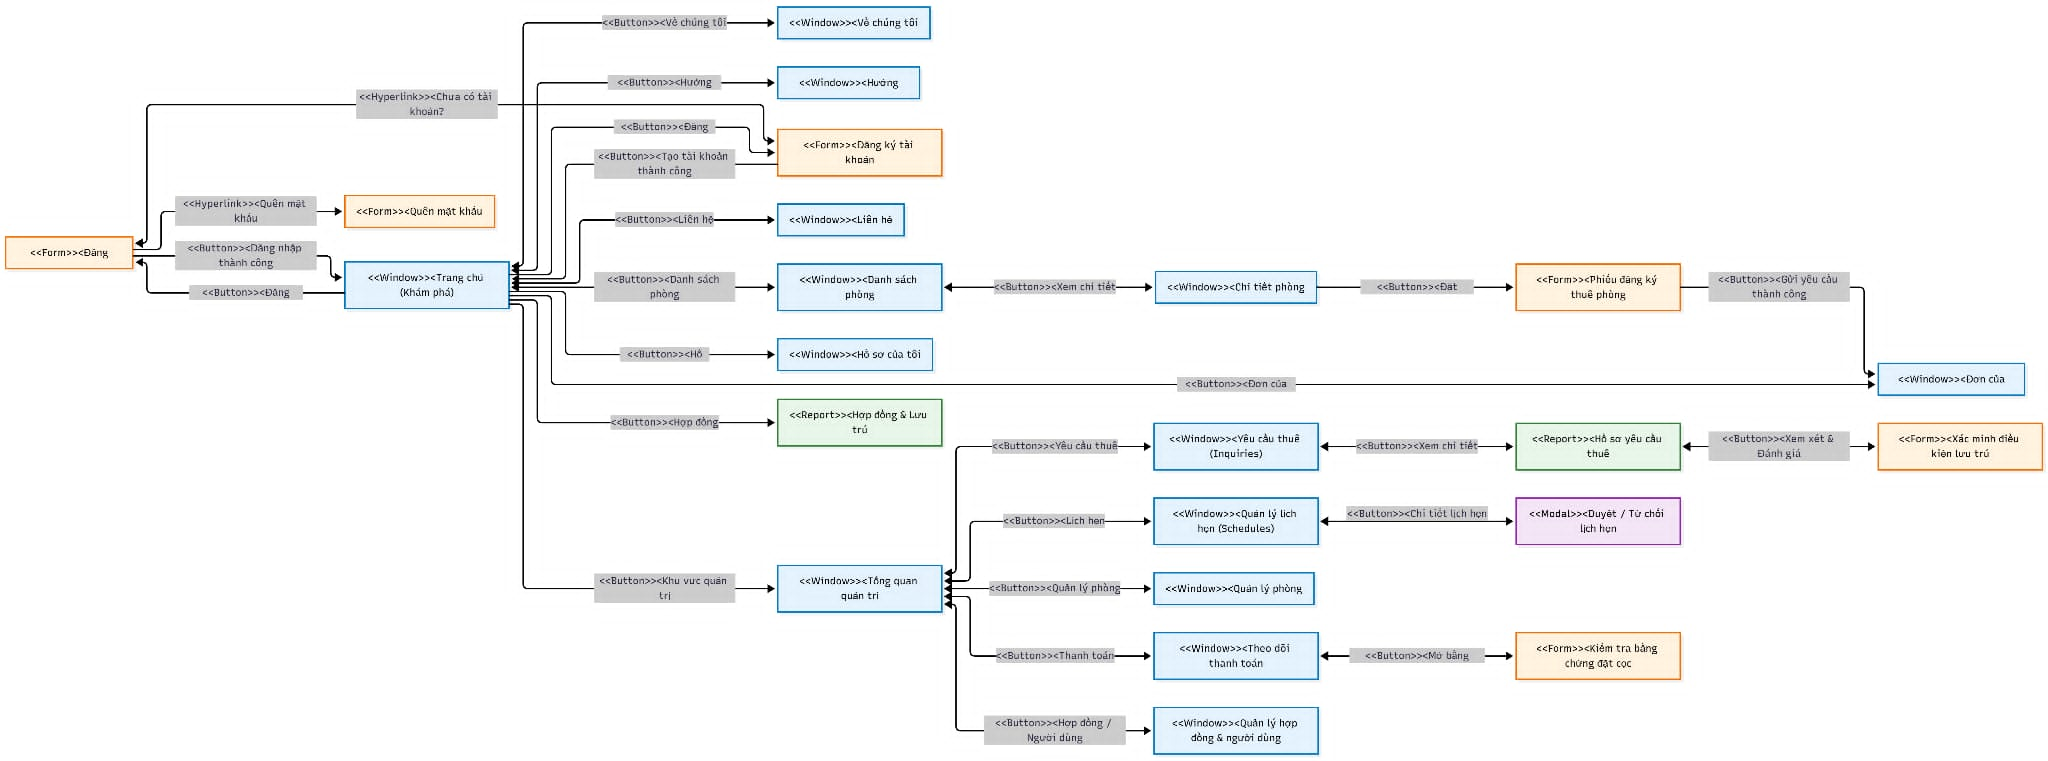
\includegraphics[width=0.98\textwidth]{images/WindowsNavigationDiagram}
    \caption{Sơ đồ điều hướng màn hình hệ thống HomeStay Dorm}
\end{figure}

\subsubsection*{Các nguyên lý thiết kế giao diện (UI Principles)}

Dựa trên cấu trúc frontend sử dụng \textbf{Angular 17/18+} và framework \textbf{Tailwind CSS}, hệ thống HomeStay Dorm tuân thủ nghiêm ngặt 4 nguyên lý thiết kế giao diện cốt lõi sau đây nhằm nâng cao trải nghiệm người dùng:

\subsubsection{Bố cục màn hình (Layout)}
Hệ thống sử dụng phương pháp phân chia khu vực (Screen Partitioning) kết hợp luồng thiết kế linh hoạt, giúp người dùng dễ dàng định vị thông tin và thao tác:
\begin{itemize}[leftmargin=*, nosep]
    \item \textbf{Vùng điều hướng (Navigation Area):} Được đặt ở thanh menu trên cùng (Navbar) đối với khu vực Public/Customer. Vùng này tự động thay đổi theo trạng thái đăng nhập, tích hợp Menu chọn ngôn ngữ (Anh/Việt) và Menu người dùng. Đối với khu vực Quản trị (Admin), hệ thống bổ sung \textbf{Sidebar bên trái} chứa các module chức năng chuyên sâu (\textit{Yêu cầu thuê, Lịch hẹn, Quản lý phòng, Thanh toán, Người dùng}).
    \item \textbf{Vùng thao tác (Workspace Area):} Không gian hiển thị trung tâm. Các biểu mẫu (\texttt{<<Form>>}) như \textit{Phiếu đăng ký thuê phòng} hay các vùng tra cứu dữ liệu (\texttt{<<Window>>}) được đặt ở trung tâm trong các thẻ (Cards) với nền bo góc, tạo đổ bóng tinh tế để tập trung tối đa sự chú ý.
    \item \textbf{Vùng thông tin \& Chân trang (Status/Footer Area):} Cung cấp các thông tin liên hệ tĩnh (Trụ sở: 227 Nguyễn Văn Cừ, Phường 4, Quận 5), các số hotline, email và giờ làm việc, hiển thị đồng nhất trên mọi màn hình.
\end{itemize}

\subsubsection{Nhận thức nội dung (Content Awareness)}
Hệ thống đảm bảo người dùng luôn biết rõ họ đang ở đâu, đang làm gì và trạng thái quy trình ra sao:
\begin{itemize}[leftmargin=*, nosep]
    \item \textbf{Tiêu đề và Phụ đề (Titles \& Subtitles):} Mỗi màn hình đều có ngữ cảnh rõ ràng. Ví dụ: Màn hình đặt phòng hiển thị \textit{``Phiếu đăng ký thuê phòng - Cho chúng tôi biết nhu cầu của bạn...''}; màn hình quản lý lịch hẹn có \textit{``Quản lý Lịch hẹn - Theo dõi và sắp xếp lịch xem phòng thực tế...''}.
    \item \textbf{Phản hồi trạng thái (State Feedback):} Tích hợp các huy hiệu (Badges) và mã màu (Color-coding) trạng thái thông minh theo thời gian thực. Ví dụ: Trạng thái \textit{Pending} dùng màu Vàng (Amber), \textit{Scheduled / Paid} dùng màu Xanh (Emerald), và \textit{Cancelled / Rejected} dùng màu Đỏ (Red). Hệ thống ánh xạ chính xác trạng thái từ Database sang UI thông qua file \texttt{vi.json}.
    \item \textbf{Chỉ báo tiến trình \& Empty State (Loading / Empty States):} Xây dựng Loading overlay toàn cục với logo và Slogan \textit{``Nurturing Your Journey, Building Your Home.''} kết hợp vòng xoay (spinner). Ngoài ra, khi không có dữ liệu, hệ thống luôn có Empty State rõ ràng (ví dụ: \textit{``Không tìm thấy lịch hẹn cho các bộ lọc đã chọn''}).
\end{itemize}

\subsubsection{Tính nhất quán (Consistency)}
\begin{itemize}[leftmargin=*, nosep]
    \item \textbf{Đồng bộ Thuật ngữ (Terminology):} Nhờ sử dụng kiến trúc đa ngôn ngữ \texttt{@ngx-translate} (file \texttt{vi.json} / \texttt{en.json}), các từ ngữ nghiệp vụ mang tính đồng nhất tuyệt đối trên mọi màn hình. Cụm từ \textit{``Chi nhánh''}, \textit{``Phòng đôi''}, \textit{``Phòng bốn''}, \textit{``Bằng chứng đặt cọc''} được dùng xuyên suốt.
    \item \textbf{Đồng bộ Tương tác (Interaction \& Visual Consistency):} Sử dụng mã màu thương hiệu \texttt{\#264893} cho các nút hành động chính (Primary Buttons). Hiệu ứng \textit{Hover} được dùng đồng nhất (class \texttt{.hover-effect}). Các thao tác quan trọng hoặc mang tính phá hủy (Từ chối, Hủy đơn, Duyệt lịch) đều sử dụng \textbf{Modal Overlay} với nền mờ tối màu để yêu cầu người dùng xác nhận lần cuối.
\end{itemize}

\subsubsection{Tối thiểu hóa nỗ lực (Minimal User Effort)}
Hệ thống được thiết kế để hạn chế tối đa số thao tác thừa, giúp người dùng làm việc nhanh chóng, hiệu quả:
\begin{itemize}[leftmargin=*, nosep]
    \item \textbf{Tự động điền dữ liệu (Prefilled Data):} Tại chức năng \textit{Đăng ký thuê phòng}, nếu khách hàng chọn Đặt phòng từ trang \textit{Chi tiết phòng}, hệ thống tự động ghi nhận \texttt{room\_id} và \texttt{branch\_name} qua Angular Router State, người dùng không cần phải chọn lại. Tương tự, tại trang \textit{Thanh toán} của Admin, Form "Tạo yêu cầu đặt cọc" tự động điền sẵn tên khách, chi nhánh, phòng và số tiền.
    \item \textbf{Luồng biểu mẫu đa bước (Wizard Form Optimization):} Biểu mẫu \textit{``Phiếu đăng ký thuê phòng''} thay vì hiển thị thành một trang dài, đã được chia nhỏ thành 4 bước (Steps) rõ ràng thông qua biến \texttt{currentPage} (Chọn phòng $\rightarrow$ Tải CCCD $\rightarrow$ Xác nhận lịch $\rightarrow$ Hoàn tất). Có thanh báo số bước giúp người dùng không bị ngợp thông tin.
    \item \textbf{Bộ lọc tự động và Tác vụ nhanh (Smart Filters \& Quick Actions):} Các màn hình tra cứu của Admin và Customer đều cung cấp thanh tìm kiếm (Search bar) debounce tự động và các Dropdown lọc theo Chi nhánh, Trạng thái (được xử lý tức thời không cần tải lại trang).
\end{itemize}
